%%%%%%%%%%%%%%%%%%%%%%%%%%%%%%%%%%%%%%%%
% Structured General Purpose Assignment
% LaTeX Template
%
% This template has been downloaded from:
% http://www.latextemplates.com
%
% Original author:
% Ted Pavlic (http://www.tedpavlic.com)
%
% Note:
% The \lipsum[#] commands throughout this template generate dummy text
% to fill the template out. These commands should all be removed when 
% writing assignment content.
%
%%%%%%%%%%%%%%%%%%%%%%%%%%%%%%%%%%%%%%%%%

%----------------------------------------------------------------------------------------
%       PACKAGES AND OTHER DOCUMENT CONFIGURATIONS
%----------------------------------------------------------------------------------------

\documentclass{article}

\usepackage{fancyhdr} % Required for custom headers
\usepackage{lastpage} % Required to determine the last page for the footer
\usepackage{extramarks} % Required for headers and footers
\usepackage{graphicx} % Required to insert images
\usepackage{lipsum} % Used for inserting dummy 'Lorem ipsum' text into the template
\usepackage{subcaption}
\usepackage{algorithm}
\usepackage{algpseudocode}
\usepackage{pifont}


\usepackage{amsmath}

% Margins
\topmargin=-0.45in
\evensidemargin=0in
\oddsidemargin=0in
\textwidth=6.5in
\textheight=9.0in
\headsep=0.25in 

\linespread{1.1} % Line spacing

% Set up the header and footer
\pagestyle{fancy}
\lhead{\hmwkAuthorName} % Top left header
\chead{\hmwkClass\ : \hmwkTitle} % Top center header
\rhead{\firstxmark} % Top right header
\lfoot{\lastxmark} % Bottom left footer
\cfoot{} % Bottom center footer
\rfoot{Page\ \thepage\ of\ \pageref{LastPage}} % Bottom right footer
\renewcommand\headrulewidth{0.4pt} % Size of the header rule
\renewcommand\footrulewidth{0.4pt} % Size of the footer rule

\setlength\parindent{0pt} % Removes all indentation from paragraphs

%----------------------------------------------------------------------------------------
%       DOCUMENT STRUCTURE COMMANDS
%       Skip this unless you know what you're doing
%----------------------------------------------------------------------------------------

% Header and footer for when a page split occurs within a problem environment
\newcommand{\enterProblemHeader}[1]{
\nobreak\extramarks{#1}{#1 continued on next page\ldots}\nobreak
\nobreak\extramarks{#1 (continued)}{#1 continued on next page\ldots}\nobreak
}

% Header and footer for when a page split occurs between problem environments
\newcommand{\exitProblemHeader}[1]{
\nobreak\extramarks{#1 (continued)}{#1 continued on next page\ldots}\nobreak
\nobreak\extramarks{#1}{}\nobreak
}

\setcounter{secnumdepth}{0} % Removes default section numbers
\newcounter{homeworkProblemCounter} % Creates a counter to keep track of the number of problems

\newcommand{\homeworkProblemName}{}
\newenvironment{homeworkProblem}[1][Problem \arabic{homeworkProblemCounter}]{ % Makes a new environment called homeworkProblem which takes 1 argument (custom name) but the default is "Problem #"
\stepcounter{homeworkProblemCounter} % Increase counter for number of problems
\renewcommand{\homeworkProblemName}{#1} % Assign \homeworkProblemName the name of the problem
\section{\homeworkProblemName} % Make a section in the document with the custom problem count
\enterProblemHeader{\homeworkProblemName} % Header and footer within the environment
}{
\exitProblemHeader{\homeworkProblemName} % Header and footer after the environment
}

\newcommand{\problemAnswer}[1]{ % Defines the problem answer command with the content as the only argument
\noindent\framebox[\columnwidth][c]{\begin{minipage}{0.98\columnwidth}#1\end{minipage}} % Makes the box around the problem answer and puts the content inside
}

\newcommand{\homeworkSectionName}{}
\newenvironment{homeworkSection}[1]{ % New environment for sections within homework problems, takes 1 argument - the name of the section
\renewcommand{\homeworkSectionName}{#1} % Assign \homeworkSectionName to the name of the section from the environment argument
\subsection{\homeworkSectionName} % Make a subsection with the custom name of the subsection
\enterProblemHeader{\homeworkProblemName\ [\homeworkSectionName]} % Header and footer within the environment
}{
\enterProblemHeader{\homeworkProblemName} % Header and footer after the environment
}
   
%----------------------------------------------------------------------------------------
%       NAME AND CLASS SECTION
%----------------------------------------------------------------------------------------

\newcommand{\hmwkTitle}{Assignment\ \#6 } % Assignment title
\newcommand{\hmwkDueDate}{Wednesday,\ December\ 2,\ 2015} % Due date
\newcommand{\hmwkClass}{CSCI-567} % Course/class
\newcommand{\hmwkClassTime}{} % Class/lecture time
\newcommand{\hmwkAuthorName}{Saket Choudhary} % Your name
\newcommand{\hmwkAuthorID}{2170058637} % Teacher/lecturer
%----------------------------------------------------------------------------------------
%       TITLE PAGE
%----------------------------------------------------------------------------------------

\title{
\vspace{2in}
\textmd{\textbf{\hmwkClass:\ \hmwkTitle}}\\
\normalsize\vspace{0.1in}\small{Due\ on\ \hmwkDueDate}\\
\vspace{0.1in}\large{\textit{\hmwkClassTime}}
\vspace{3in}
}

\author{\textbf{\hmwkAuthorName} \\
        \textbf{\hmwkAuthorID}
        }
\date{} % Insert date here if you want it to appear below your name

%----------------------------------------------------------------------------------------

\begin{document}

\maketitle

%----------------------------------------------------------------------------------------
%       TABLE OF CONTENTS
%----------------------------------------------------------------------------------------

%\setcounter{tocdepth}{1} % Uncomment this line if you don't want subsections listed in the ToC

\newpage
\tableofcontents
\newpage








\begin{homeworkProblem}[Problem 1.1] % Custom section title
\begin{homeworkSection}{\homeworkProblemName: ~(a)}

\problemAnswer{
	\begin{align*}
	J &= \frac{1}{N} \sum_{i=1}^N (x_i -p_{i1}e_i -p_{i2}e_2)^T(x_i -p_{i1}e_i -p_{i2}e_2)
	\end{align*}
	
	Let's define $k_i = x_i-p_{i1}$.
	\begin{align*}
	J &= \frac{1}{N} \sum_{i=1}^N (k_i-p_{i2}e_2)^T(k_i-p_{i2}e_2)\\
	&= = \frac{1}{N} \sum_{i=1}^N (k_i^Tk_i - p_{i2}k_i^te_2-p_{i2}e_2^Tk_i + p_{i2}^2e_2^Te_2)\\
	\frac{\partial J}{\partial p_{i2}} &=  \frac{1}{N} \sum_{i=1}^N (0-k_i^Te_2-e_2^Tk_i + 2p_{i2}e_2^Te_2)\\
	&= \frac{1}{N} \sum_{i=1}^N (-2e_2^Tk_i+2p_{i2})
	\end{align*}
	
	\begin{eqnarray*}
	\frac{\partial J}{\partial p_{i2}} = 0 \\
	\implies \frac{1}{N} \sum_{i=1}^N (-2e_2^Tk_i+2p_{i2}) = 0\\
	\implies p_{i2} = e_2^Tk_i \forall i \\
	\implies p_{i2} = e_2^T(x_i-p_{i1}e_1)\\
	\implies p_{i2} = e_2^Tx_i 
	\end{eqnarray*}
}
\end{homeworkSection}

\begin{homeworkSection}{\homeworkProblemName: ~(b)}
	
	\problemAnswer{
		\begin{align*}
		\tilde{J} &= -e_2^TSe_2 + \lambda_2(e_2^Te_2-1)+\lambda_{12}(e_2^Te_1-0)\\
		\frac{\partial \tilde{J}}{\partial e_2} &= -(S+S^T)e_2 + 2 \lambda_2 e_2 + \lambda_{12}e_1\\
		&=-2Se_2+2\lambda_2e_2+\lambda_{12}e_1\ \text{since $S=S^T$}
		\end{align*}
		
		\begin{eqnarray*}
			\frac{\partial \tilde{J}}{\partial e_2} = 0\\
			\implies -2Se_2+2\lambda_2e_2+\lambda_{12}e_1 = 0\\
			\implies -2e_1^TSe_2+2\lambda_2 e_1^Te_2 + \lambda_{12} e_1^Te_1 = 0 \ \text{ pre multipllying $e_1^T$}\\
			\implies -2(Se_1)^Te_2+ 2 \lambda_2\times 0 + \lambda_{12} \times 1 = 0\ \text{since $S=S^T$}\\
			\implies \lambda_{12} = 0\ \text{Since $ (Se_1)^Te_2 = 0$}\\
			\implies Se_2 = \lambda_2e_2
		\end{eqnarray*}
		Thus, the value of $e_2$ minimising $\tilde{J}$ is given by second largest eigenvector of $S$. $Se_2 = \lambda_2 e_2$
}
\end{homeworkSection}
\end{homeworkProblem}


\begin{homeworkProblem}[Problem 1.2] % Custom section title
	\begin{homeworkSection}{\homeworkProblemName: ~(a)}
		
		\problemAnswer{
			\begin{align*}
			||x_i-\sum_{j=1}^K p_{ij}e_j||_2^2 &= (x_i-\sum_{j=1}^K p_{ij}e_j)^T(x_i-\sum_{j=1}^K p_{ij}e_j)\\
			&= (x_i^T- \sum_{j=1}^Kp_{ij}e_j^T)(x_i-\sum_{j=1}^K p_{ij}e_j)\\
			&= x_i^T-x_i^T - \sum_{j=1}^Kp_{ij}x_i^Te_j -   \sum_{j=1}^Kp_{ij}e_j^Tx_i+  \sum_{j,k}p_{ij}e_j^Te_kp_{ik}\\
			&= x_i^Tx_i - \sum_{j=1}^K e_j^Tx_ix_i^Te_j - \sum_{j=1}^K e_j^Tx_ix_i^Te_j + \sum_{j=1}^K p_{ij}e_j^Te_jp_{ij} \ \text{since $e_j^Te_k=0$ for $k\neq m$}\\
			&= x_i^Tx_i - \sum_{j=1}^K e_j^Tx_ix_i^Te_j - \sum_{j=1}^K e_j^Tx_ix_i^Te_j +  \sum_{j=1}^K e_j^T x_i x_it^Te_j\\
			& = x_i^Tx_i - \sum_{j=1}^K e_j^Tx_ix_i^Te_j
			\end{align*}
		}
	\end{homeworkSection}
	
	\begin{homeworkSection}{\homeworkProblemName: ~(a)}
		
		\problemAnswer{
			\begin{align*}
			J_K &= \frac{1}{N} \sum_{i=1}^N (x_i^Tx_i-\sum_{j=1}^Ke_j^Tx_ix_i^Te_j)\\
			&=\frac{1}{N} \sum_{i=1}^N (x_i^Tx_i-\sum_{j=1}^Ke_j^TSe_j)\\
			&=\frac{1}{N} \sum_{i=1}^N (x_i^Tx_i-\sum_{j=1}^Ke_j^T\lambda_j e_j)\\
			&= \frac{1}{N} \sum_{i=1}^N (x_i^Tx_i)- \frac{1}{N} \sum_{i=1}^N(\sum_{j=1}^K\lambda_j)\ \text{since $e_j^Te_j=1$}\\
			&=  \frac{1}{N} \sum_{i=1}^N (x_i^Tx_i) - \frac{1}{N}N \sum_{j=1}^K\lambda_j \\
			&=  \frac{1}{N} \sum_{i=1}^N (x_i^Tx_i) -  \sum_{j=1}^K\lambda_j
			\end{align*}
		}
	\end{homeworkSection}
	
	\begin{homeworkSection}{\homeworkProblemName: ~(c)}
		
		\problemAnswer{
			Error from only using $K$ components instead of $D$. It is easy to realise when we have $K=D$ components, $J_D=0$ since there are no missing components. 
			In case $K<D$, error arises due to missing components, where missing components include eigenvectors from $K+1$ to $D$.
			\begin{align*}
			J_D &= \frac{1}{N} \sum_{i=1}x_i^Tx_i - \sum_{j=1}^D \lambda_j \\
			& = 0 \\
			J_K &= \frac{1}{N} \sum_{i=1}x_i^Tx_i  - \sum_{j=1}^K \lambda_j \\
			&=  (\frac{1}{N} \sum_{i=1}x_i^Tx_i - \sum_{j=1}^D \lambda_j) + \sum_{j=D+1}^K \lambda_j\\
			& = 0+\sum_{j=D+1}^K \lambda_j\\
			&= \sum_{j=D+1}^K \lambda_j
			\end{align*}
		}
	\end{homeworkSection}
\end{homeworkProblem}
	
\begin{homeworkProblem}[Problem 2] % Custom section title
		\begin{homeworkSection}{\homeworkProblemName: ~(a)}
			

	\problemAnswer{
		$$
		a = \begin{matrix}
		0.8 & 0.2\\
		0.4 & 0.6\\
		\end{matrix}
		$$
		
		Given $O=AGCGTA$
		
		\textbf{a}:
		$P(O;\theta) = \sum_{j=1}^2 \alpha_6(j)$
		
		Where $\alpha_t(j) = P(O_t|S_t=j)\sum_{i=1}^2a_{ij}\alpha_{t-1}(j)$
		
		$\alpha_1(j) = P(O_1|S_1=j)P(S_1=j)$
		
		And for $i>1$
		$\alpha_t(j) = P(O_t|S_t=j) \times \sum_{i} a_{ij} \alpha_{t-1}(j)$
		Thus,
		\begin{eqnarray*}
		\alpha_1(1) = P(S_1=1)P(O_1|S_1=1) = \pi_1 \times p_{1a} = 0.7 \times 0.4 = 0.28\\
		\alpha_1(2) = \pi_2 \times p_{2a} = 0.3 \times 0.2 = 0.06\\
		\alpha_2(1) = P(O_2|S_2=1) \times \sum_{i}a_{i1} \alpha_1(j) = b_{1g} \times (a_{11}\alpha_1(1) + a_{21}\alpha_1(2)) = 0.0992\\
		\alpha_2(2) = b_{2g} \times (a_{12}\alpha_1(1) + a_{22}\alpha_1(2)) = 0.0184\\
		\alpha_3(1) = b_{1c} \times (a_{11}\alpha_2(1) + a_{21}\alpha_2(2)) = 0.008672\\
		\alpha_3(2) = b_{2c} \times (a_{12}\alpha_2(1) + a_{22}\alpha_2(2)) = 0.009264\\
		\alpha_4(1) = b_{1g} \times (a_{11}\alpha_3(1) + a_{21}\alpha_3(2)) = 0.00425\\
		\alpha_4(2) = b_{2g} \times (a_{12}\alpha_3(1) + a_{22}\alpha_3(2)) = 0.0014585\\
		\alpha_5(1) = b_{1t} \times (a_{11}\alpha_4(1) + a_{21}\alpha_4(2)) = 0.000398\\
		\alpha_5(2) = b_{2t} \times (a_{12}\alpha_4(1) + a_{22}\alpha_4(2)) = 0.0005179\\
		\alpha_6(1) = b_{1a} \times (a_{11}\alpha_5(1) + a_{21}\alpha_5(2)) = 0.0002105\\
		\alpha_6(2) = b_{2a} \times (a_{12}\alpha_5(1) + a_{22}\alpha_5(2)) = 0.00007810 \\		
		\end{eqnarray*}
		
		$P(O; \theta) = \alpha_6(1) + \alpha_6(2) = 0.0002886$ 
		
 	
		}
			\end{homeworkSection}
			
		\begin{homeworkSection}{\homeworkProblemName: ~(b)}
			\problemAnswer{
				
				I refer to hidden states $S_1, S_2$ as 1,2 respectively.
				$\beta_{t-1}(i) = \sum_{j=1}^2 \beta_{t}a_{ij}P(O_t|X_t=S_j)$
				
				\begin{eqnarray*}
					\beta_6(1) = 1\\
					\beta_6(2) = 1\\
					\beta_5(1) = \beta_6(1)a_{11}b_{1a} + \beta_6(2)a_{12}b_{2} = 0.36\\
					\beta_5(2) = \beta_6(1)a_{21}b_{1a} + \beta_6(2)a_{22}b_{2a} = 0.28\\
					\beta_4(1) = \beta_5(1)a_{11}b_{1t} + \beta_5(2)a_{12}b_{2} = 0.0456 \\
					\beta_4(2) = \beta_5(1)a_{21}b_{1t} + \beta_5(2)a_{22}b_{2a} = 0.0648
				\end{eqnarray*}
				
				\begin{eqnarray*}
				P(X_6=S_i | O, \theta) = \frac{\alpha_6(S_i)\beta_6(S_i)}{\alpha_6(S_1)\beta_6(S_1)+\alpha_6(S_2)\beta_6(S_2)}
				\end{eqnarray*}
				
				Thus,
				\begin{align*}
				P(X_6=S_1 | O, \theta) &= \frac{\alpha_6(S_1)\beta_6(S_1)}{\alpha_6(S_1)\beta_6(S_1)+\alpha_6(S_2)\beta_6(S_2)}\\
				&= \frac{0.0002105}{0.0002886}\\
				&= 0.7293\\
				P(X_6=S_2 | O, \theta) &= \frac{\alpha_6(S_2)\beta_6(S_2)}{\alpha_6(S_1)\beta_6(S_1)+\alpha_6(S_2)\beta_6(S_2)}\\
				&= \frac{0.000078}{0.0002886} \\
				&= 0.2702
				\end{align*}
				
				}
		\end{homeworkSection}
		\begin{homeworkSection}{\homeworkProblemName: ~(b)}
			\problemAnswer{
				\begin{align*}
				P(X_4=S_1 | O, \theta) &= \frac{\alpha_4(S_1)\beta_4(S_1)}{\alpha_4(S_1)\beta_4(S_1)+\alpha_4(S_2)\beta_4(S_2)}\\
				&= \frac{0.0456}{0.1104}\\
				&= 0.413\\
				P(X_4=S_2 | O, \theta) &= \frac{\alpha_4(S_2)\beta_4(S_2)}{\alpha_4(S_1)\beta_4(S_1)+\alpha_4(S_2)\beta_4(S_2)}\\
				&= \frac{0.0648}{0.1104} \\
				&= 0.587
				\end{align*}
			}
		\end{homeworkSection}

		\begin{homeworkSection}{\homeworkProblemName: ~(d)}
			\problemAnswer{
				$\delta_t(j) = \max_i \delta_{t-1}(i) a_{ij} P(x_t|Z_t=s_i)$
				
				\begin{eqnarray*}
				\delta_1(1) = \pi_1 b_{1a} = 0.28\\
				\delta_1(2) = \pi_2 b_{2a} = 0.06\\
				\delta_2(1) = b_{1g} \times max(\delta_1(1)a_{11}, \delta_1(2)a_{21}) = 0.896\\
				\delta_2(2) =  b_{2g} \times max(\delta_1(1)a_{12}, \delta_1(2)a_{22}) = 0.072\\
				\delta_3(1) = b_{1c} \times (\delta_2(1)a_{11} + \delta_2(2)a_{21} )\\
				\end{eqnarray*}

					}
			\end{homeworkSection}
		\begin{homeworkSection}{\homeworkProblemName: ~(e)}
			\problemAnswer{
				$O_7 = \arg \max_O P(O|O\theta)$
				
				\begin{align*}
				P(O_7|O) &= \sum_{i=1}^2 P(O_7,X_7=S_i|O)\\
				&=  \sum_{i=1}^2 P(O_7|X_7=S_i) \times \sum_{j=1}^2 P(X_7=S_i,X_6=S_j|O)\\
				&=  \sum_{i=1}^2 P(O_7|X_7=S_i) \times \sum_{j=1}^2 P(X_7=S_i|X_6=S_j) P(X_6=S_j|O)\\
				& = b_{1k} \times (P(X_6=S_1|\theta)\times a_{11} + P(X_6=S_2|\theta) \times a_{21}) \\ &+ b_{2k} \times (P(X_6=S_1|\theta)\times a_{12} + P(X_6=S_2|\theta) \times a_{22})\ where\  k \in (A,C,T,G)
				\end{align*}
				
				Define $c_1 = P(X_6=S_1|\theta)\times a_{11} + P(X_6=S_2|\theta) \times a_{21} = 0.6915$
				
				Define,$c_2 = P(X_6=S_1|\theta)\times a_{12} + P(X_6=S_2|\theta) \times a_{22} = 0.307 $

		Thus, $P(O_7=k|\theta) = 0.6915b_{1k}  + 0.307b_{2k} $

		
		
		\begin{eqnarray*}
		P(O_7=A|\theta) = 0.6915*0.4+0.307*0.2 = 0.338\\
		P(O_7=T|\theta) = 0.6915*0.1+0.307*0.3 = 0.16125\\
		P(O_7=C|\theta) = 0.6915*0.1+0.307*0.3 = 0.16125\\
		P(O_7=G|\theta) = 0.6915*0.4+0.307*0.2 = 0.338\\
 		\end{eqnarray*}						
			
			Thus, $A,G$ are equiprobable as $7^{th}$ observed sequence.	
			}
		\end{homeworkSection}
						
\end{homeworkProblem}		
\newpage

\begin{homeworkProblem}[Problem 3.1] % Custom section title
\begin{homeworkSection}{\homeworkProblemName : ~(b)}
		\begin{figure}
	\begin{minipage}{0.2\linewidth}
		
\includegraphics[width=\linewidth]{eig-1}	
		\caption{PC-1}
	\end{minipage}
	\begin{minipage}{0.2\linewidth}
		
\includegraphics[width=\linewidth]{eig-2}	
		\caption{PC-2}
	\end{minipage}
	\begin{minipage}{0.2\linewidth}
		
\includegraphics[width=\linewidth]{eig-3}	
		\caption{PC-3}
	\end{minipage}
	\begin{minipage}{0.2\linewidth}
		
\includegraphics[width=\linewidth]{eig-4}	
		\caption{PC-4}
	\end{minipage}
		\end{figure}
		
		\begin{figure}
			\begin{minipage}{0.2\linewidth}
				
\includegraphics[width=\linewidth]{eig-5}	
				\caption{PC-5}
			\end{minipage}
			\begin{minipage}{0.2\linewidth}
				
\includegraphics[width=\linewidth]{eig-6}	
				\caption{PC-6}
			\end{minipage}
			\begin{minipage}{0.2\linewidth}
				
\includegraphics[width=\linewidth]{eig-7}	
				\caption{PC-7}
			\end{minipage}
			\begin{minipage}{0.2\linewidth}
				
\includegraphics[width=\linewidth]{eig-8}	
				\caption{PC-8}
			\end{minipage}
		\end{figure}
\end{homeworkSection}

\newpage

\begin{homeworkSection}{\homeworkProblemName : ~(c)}
		\begin{figure}
			\begin{minipage}{0.15\linewidth}
				
\includegraphics[width=\linewidth]{3c-orig-5500}	
				\caption{\#5500 Original}
			\end{minipage}
			\begin{minipage}{0.15\linewidth}
				
\includegraphics[width=\linewidth]{3c-5500-1}	
				\caption{\#5500 K-1}
			\end{minipage}
			\begin{minipage}{0.15\linewidth}
				
\includegraphics[width=\linewidth]{3c-5500-5}	
				\caption{\#5500 K-5}
			\end{minipage}
			\begin{minipage}{0.15\linewidth}
				
\includegraphics[width=\linewidth]{3c-5500-10}	
				\caption{\#5500 K-10}
			\end{minipage}
			\begin{minipage}{0.15\linewidth}
				
\includegraphics[width=\linewidth]{3c-5500-20}	
				\caption{\#5500 K-20}
			\end{minipage}
			\begin{minipage}{0.18\linewidth}
				
\includegraphics[width=\linewidth]{3c-5500-80}	
				\caption{\#5500 K-80}
			\end{minipage}
		\end{figure}
		
		\begin{figure}
			\begin{minipage}{0.15\linewidth}
				
\includegraphics[width=\linewidth]{3c-orig-6500}	
				\caption{\#6500 Original}
			\end{minipage}
			\begin{minipage}{0.15\linewidth}
				
\includegraphics[width=\linewidth]{3c-6500-1}	
				\caption{\#6500 K-1}
			\end{minipage}
			\begin{minipage}{0.15\linewidth}
				
\includegraphics[width=\linewidth]{3c-6500-5}	
				\caption{\#6500 K-5}
			\end{minipage}
			\begin{minipage}{0.15\linewidth}
				
\includegraphics[width=\linewidth]{3c-6500-10}	
				\caption{\#6500 K-10}
			\end{minipage}
			\begin{minipage}{0.15\linewidth}
				
\includegraphics[width=\linewidth]{3c-6500-20}	
				\caption{\#6500 K-20}
			\end{minipage}
			\begin{minipage}{0.18\linewidth}
				
\includegraphics[width=\linewidth]{3c-6500-80}	
				\caption{\#6500 K-80}
			\end{minipage}
		\end{figure}
		
		\begin{figure}
			\begin{minipage}{0.15\linewidth}
				
\includegraphics[width=\linewidth]{3c-orig-7500}	
				\caption{\#7500 Original}
			\end{minipage}
			\begin{minipage}{0.15\linewidth}
				
\includegraphics[width=\linewidth]{3c-7500-1}	
				\caption{\#7500 K-1}
			\end{minipage}
			\begin{minipage}{0.15\linewidth}
				
\includegraphics[width=\linewidth]{3c-7500-5}	
				\caption{\#7500 K-5}
			\end{minipage}
			\begin{minipage}{0.15\linewidth}
				
\includegraphics[width=\linewidth]{3c-7500-10}	
				\caption{\#7500 K-10}
			\end{minipage}
			\begin{minipage}{0.15\linewidth}
				
\includegraphics[width=\linewidth]{3c-7500-20}	
				\caption{\#7500 K-20}
			\end{minipage}
			\begin{minipage}{0.18\linewidth}
				
\includegraphics[width=\linewidth]{3c-7500-80}	
				\caption{\#7500 K-80}
			\end{minipage}
		\end{figure}
		
		\begin{figure}
			\begin{minipage}{0.15\linewidth}
				
\includegraphics[width=\linewidth]{3c-orig-8000}	
				\caption{\#8000 Original}
			\end{minipage}
			\begin{minipage}{0.15\linewidth}
				
\includegraphics[width=\linewidth]{3c-8000-1}	
				\caption{\#8000 K-1}
			\end{minipage}
			\begin{minipage}{0.15\linewidth}
				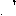
\includegraphics[width=\linewidth]{3c-8000-5}	
				\caption{\#8000 K-5}
			\end{minipage}
			\begin{minipage}{0.15\linewidth}
				
\includegraphics[width=\linewidth]{3c-8000-10}	
				\caption{\#8000 K-10}
			\end{minipage}
			\begin{minipage}{0.15\linewidth}
				
\includegraphics[width=\linewidth]{3c-8000-20}	
				\caption{\#8000 K-20}
			\end{minipage}
			\begin{minipage}{0.18\linewidth}
				
\includegraphics[width=\linewidth]{3c-8000-80}	
				\caption{\#8000 K-80}
			\end{minipage}
		\end{figure}
		\begin{figure}
			\begin{minipage}{0.15\linewidth}
				
\includegraphics[width=\linewidth]{3c-orig-8500}	
				\caption{\#8500 Original}
			\end{minipage}
			\begin{minipage}{0.15\linewidth}
				
\includegraphics[width=\linewidth]{3c-8500-1}	
				\caption{\#8500 K-1}
			\end{minipage}
			\begin{minipage}{0.15\linewidth}
				
\includegraphics[width=\linewidth]{3c-8500-5}	
				\caption{\#8500 K-5}
			\end{minipage}
			\begin{minipage}{0.15\linewidth}
				
\includegraphics[width=\linewidth]{3c-8500-10}	
				\caption{\#8500 K-10}
			\end{minipage}
			\begin{minipage}{0.15\linewidth}
				
\includegraphics[width=\linewidth]{3c-8500-20}	
				\caption{\#8500 K-20}
			\end{minipage}
			\begin{minipage}{0.18\linewidth}
				
\includegraphics[width=\linewidth]{3c-8500-80}	
				\caption{\#8500 K-80}
			\end{minipage}
		\end{figure}
\end{homeworkSection}
\begin{homeworkSection}{\homeworkProblemName : ~(d)}
	\problemAnswer{
			\begin{tabular}{|c|c|c|c|}
				\hline \#PC & Training Accuracy &  Test Accuracy & Time taken(s)  \\ 
				\hline  1 & 0.516778  & 0.122500  & 32.125276 \\ 
				\hline  5 & 0.890889  &  0.434000 &  17.126630 \\ 
				\hline  10 & 0.947333 & 0.635500 & 14.667870 \\ 
				\hline  20 & 0.947556 & 0.742500 & 14.161249  \\ 
				\hline  80& 0.920444  & 0.763500  & 17.982115 \\ 
				\hline 
			\end{tabular} 
			
			Thus we see that the training accuracy increases as the number pf principal components increase. This is intuitive since we have more information with higher principal components. Training accuracy decreases for 80 principal components  over 20 indicating that the next 60 principal components are not distinctive enough. The testing accuracy continuously increases as number of principal components increase indicating higher information gain by increasing the number of principal components.
			
			The time taken by Decision tree classifier decreases as the number of principal components increase. This is expected since there is limited information available with say 1 principal component and hence the decision tree will keep on growing in depth. whereas when higher number of PCs are used the tree depth will be smaller since there is more information at each branching step.
			
		}
\end{homeworkSection}
\end{homeworkProblem}		

\begin{homeworkProblem}[Problem 3.2] % Custom section title
	\begin{homeworkSection}{\homeworkProblemName : ~(a)}
		\problemAnswer{
			Length of shortest trace: 109\\
			Length of longest trace: 435\\
			How many different observations: 22
			}
	\end{homeworkSection}
	\begin{homeworkSection}{\homeworkProblemName : ~(a)}
		\problemAnswer{
			Hidden States: S\\
			Observations: $O^{(1)}, O^{(2)} \dots O^{(D)}$ where $O^{(i)}$ denotes the the $i^{th}$ training sample.
			$\theta = \{\pi_i, a_{ij}, b_{ik}\}$
			
			Let $T_i$ denote the trace length of $i^{th}$ training sample.
		
			Thus, any observation $O^{(i)} = \{O^{(i)}_1, O^{(i)}_2 \dots O^{(i)}_{T_i} \}$
			
			\begin{align*}
			L_D(\theta, A, B) &= \sum_{i=1}^D \log( P( O^{(i)}_1, O^{(i)}_1, \dots O^{(i)}_{T_i}, S^{(i)}_1, S^{(i)}_2, \dots S^{(i)}_{T_i} ) )\\
			&= \sum_{i=1}^D  (\log (P(S^{(i)}_1, S^{(i)}_2, \dots S^{(i)}_{T_i} ) +  P( O^{(i)}_1, O^{(i)}_1, \dots O^{(i)}_{T_i}| S^{(i)}_1, S^{(i)}_2, \dots S^{(i)}_{T_i} ) )) \\
			&= \sum_{i=1}^D \log(P(S_1^{(i)})+ \sum_{i=1}^D\sum_{t=2}^{T_i} \log(P(S_t^{(i)}|S_{t-1}^{(i)}) ) + \sum_{i=1}^D \sum_{t=1}^{T_i}\log(P(O^{(i)}_t|S^{(i)}_t)))\\
			&= \sum_{i=1}^D \log(P(S_1^{(i)})+ \sum_{i=1}^D\sum_{t=2}^{T_i} \log(P(S_t^{(i)}|S_{t-1}^{(i)}) ) + \sum_{i=1}^D \sum_{t=1}^{T_i}\log(P(O^{(i)}_t|S^{(i)}_t)))\\
			&= \sum_{i=1}^D \log(\pi_{S_1}^{(i)})  + \sum_{i=1}^D \sum_{t=2}^{T_i} \log(A^{(i)}_{t-1,t} + \sum_{i=1}^D \sum_{t=2}^{T_i} \log(B^{(i)}_{S_t^{(i)}O^{(i)}_t})
			\end{align*}
			
			Note $B^{(i)}_{S_t^{(i)}O^{(i)}_t}$ denotes the emission probability when state is $S_t^{(i)}$ and emission is $O_t^{(i)}$
				}
	\end{homeworkSection}
	
\begin{homeworkSection}{\homeworkProblemName : ~(a)}
	\problemAnswer{
		Let $S'$ denote the set of all possiblities that $S_t^{(i)}$ can take,
		
		\begin{align*}
		Q(\theta, \theta^s) &= \sum_{S \in S'} L_D(\theta,s, A,B) \times P(s| O;\theta)\\
		&= \sum_{S \in S'} \sum_{i=1}^D \log(\pi_{S_1}^{(i)})  + \sum_{S \in S'}\sum_{i=1}^D \sum_{t=2}^{T_i} \log(A^{(i)}_{t-1,t} + \sum_{S \in S'}\sum_{i=1}^D \sum_{t=2}^{T_i} \log(B^{(i)}_{S_t^{(i)}O^{(i)}_t})\\
		\end{align*}
		
		Now define the total number of hidden states to be M. 
		
		Given constraints (for each training dataset):
		\begin{align*}
		\sum_i \pi_i &=1 \\
		\sum_j A_{ij} &= 1\\
		\sum_j B_{ij} &=1\\
		\end{align*}
		Then we define a langragian as follows:
		
		\begin{align*}
		L(\theta, \theta^s) = Q(\theta, \theta^s) - \lambda_\pi(\sum_{i=1}^M \pi_i -1 ) + \sum){i=1}^M \lambda_{A_i}(\sum_{j=1}^M\lambda A_{ij} -1) - \sum_{i=1}^M \lambda_{B_i}(\sum_{j=1}^M B_{ij}- 1)\\
		\end{align*}
		
		Now, 
			 \begin{align*}
		\frac{\partial L}{\partial \pi_{S_i}}  &= 0\\
		&= \frac{\partial }{\partial \pi_{S_i}} (\sum_{S\in S'} \sum_{i=d}^D \sum_{j=1}^M \log (\pi_{S_i}) P(S_1^{(i)} = j,O;\theta)  - \lambda_\pi = 0 \\
		&=  \sum_{i=1}^D \frac{P(S_1^{(i)}=j, O;\theta)}{\pi_{S_i}} - \lambda_\pi = 0
		\end{align*}
		
		Since the likelihood is linear in terms of probability, the M step involves a posterior calculation:
		\begin{align*}
		\pi_{S_i} &= \frac{\sum_{i=1}^D P(S_1^{(i)}=S_i, O; \theta) }{ \sum_{i=d}^D \sum_{j=1}^M \sum_{i=1}^D P(S_1^{(i)}=S_i, O; \theta) }
		\end{align*}
		
	}	
\end{homeworkSection}

\end{homeworkProblem}

\end{document}
